\section{Absorptionsverhalten von Aluminium und Papier}
%kurz das ziel dieses versuchsteiles ansprechen, damit keine zwei �berschriften direkt �bereinander stehen!
%bei schwierigeren versuchen kann auch der theoretische hintergrund erl�utert werden. (mit formeln, herleitungen und erkl�rungen)
In diesem Versuchsabschnitt soll das Absorptionsverhalten von Aluminium und Papier untersucht werden.

\subsection{Versuchsdurchf�hrung}
Es wird der selbe Aufbau wie in Abschnitt \ref{sec:energieverlust} verwendet. Zwischen Quelle und Detektor werden Papier bzw. Aluminium gelegt um die Absorption zu untersuchen. Zur Verf�gung stehen Papier mit 103$\mu$m und 32$\mu$m, sowie Aluminiumfolie mit einer Dicke von 13$\mu$m. Vor der Messung wird die Kammer auf 35 Torr evakuiert.

\subsection{Auswertung}

Die aufgenommenen Spektren sind in Abb. \ref{fig:ab_alu} (Aluminium), Abb. \ref{fig:ab_papier} (Papier) und Abb. \ref{fig:ab_biebel} (Biebelpapier) zu sehen. Die Alufolie schw�cht die $\alpha$-Strahlung ab, was an der Verschiebung nach links zu sehen ist. Das normale Papier Block die Strahlung nahezu vollst�ndig ab. Bei der Absorbtion durch das Biebelpapier, werde die ersten der Peaks zu einem verwaschen.


\begin{figure}[H]
	\centering
  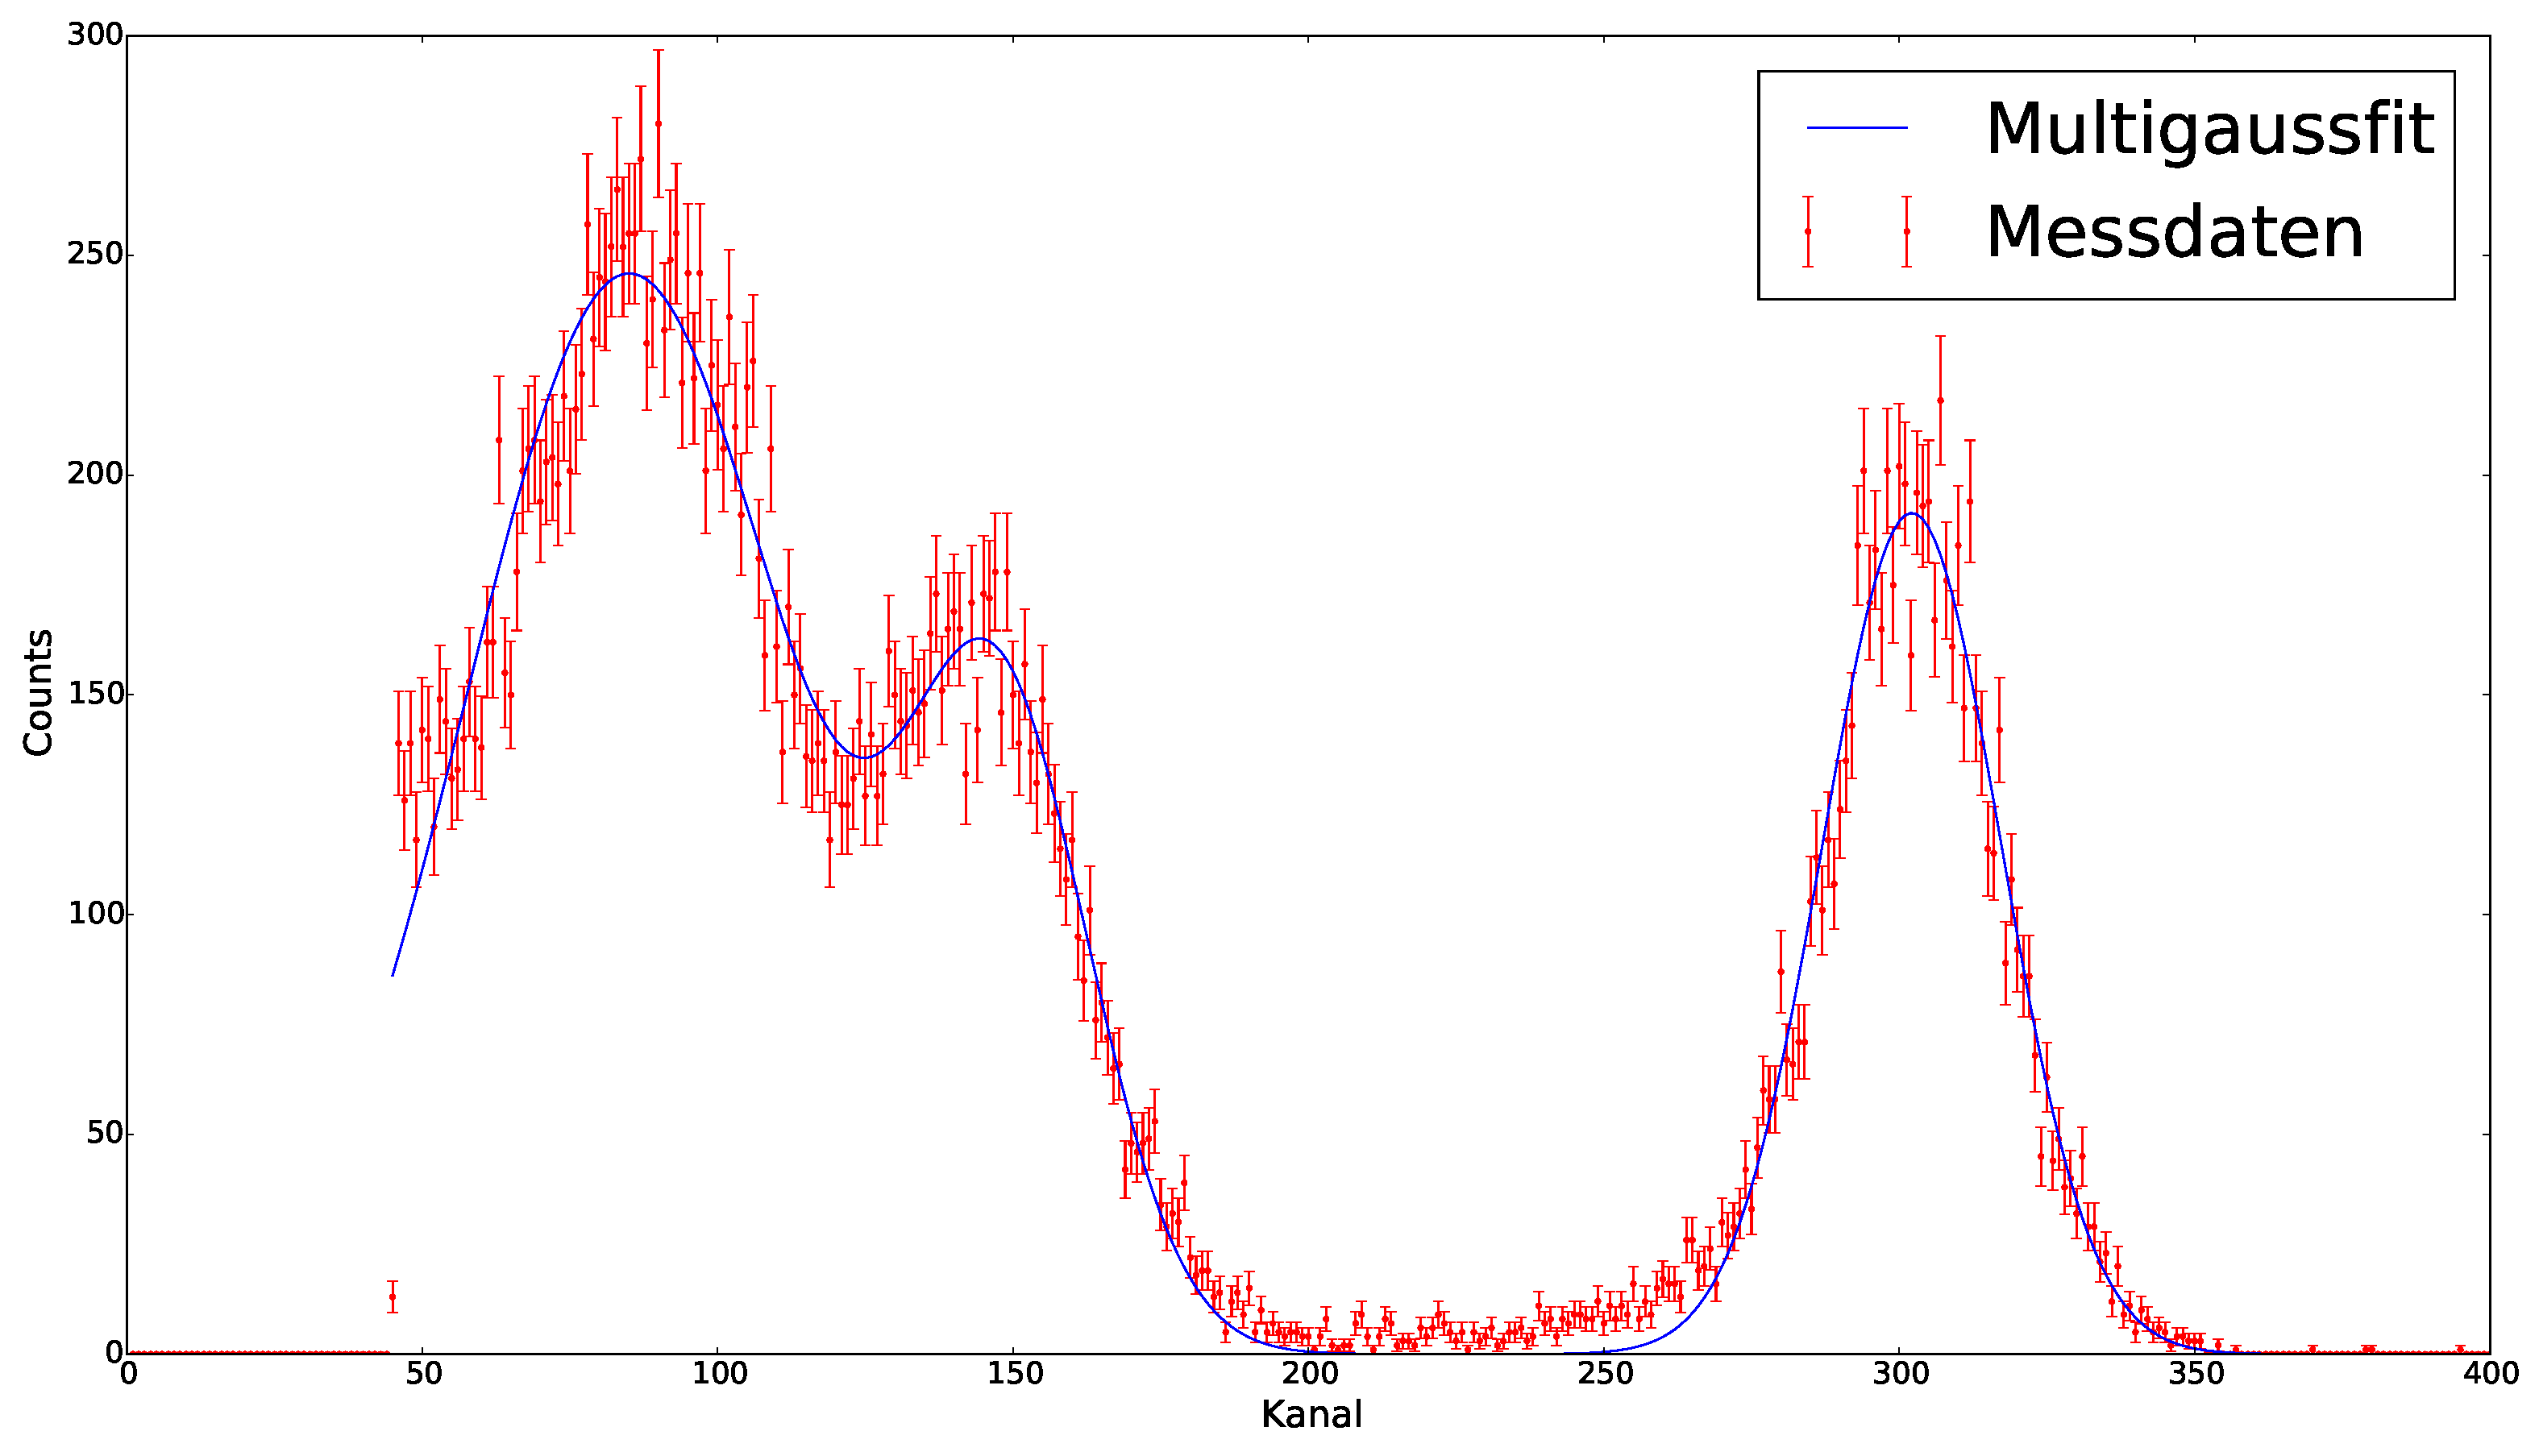
\includegraphics[scale=0.2]{ab_alu.pdf}
	\caption{Schematischer Aufbau des Streukammer}
	\label{fig:ab_alu}
\end{figure}

\begin{figure}[H]
	\centering
  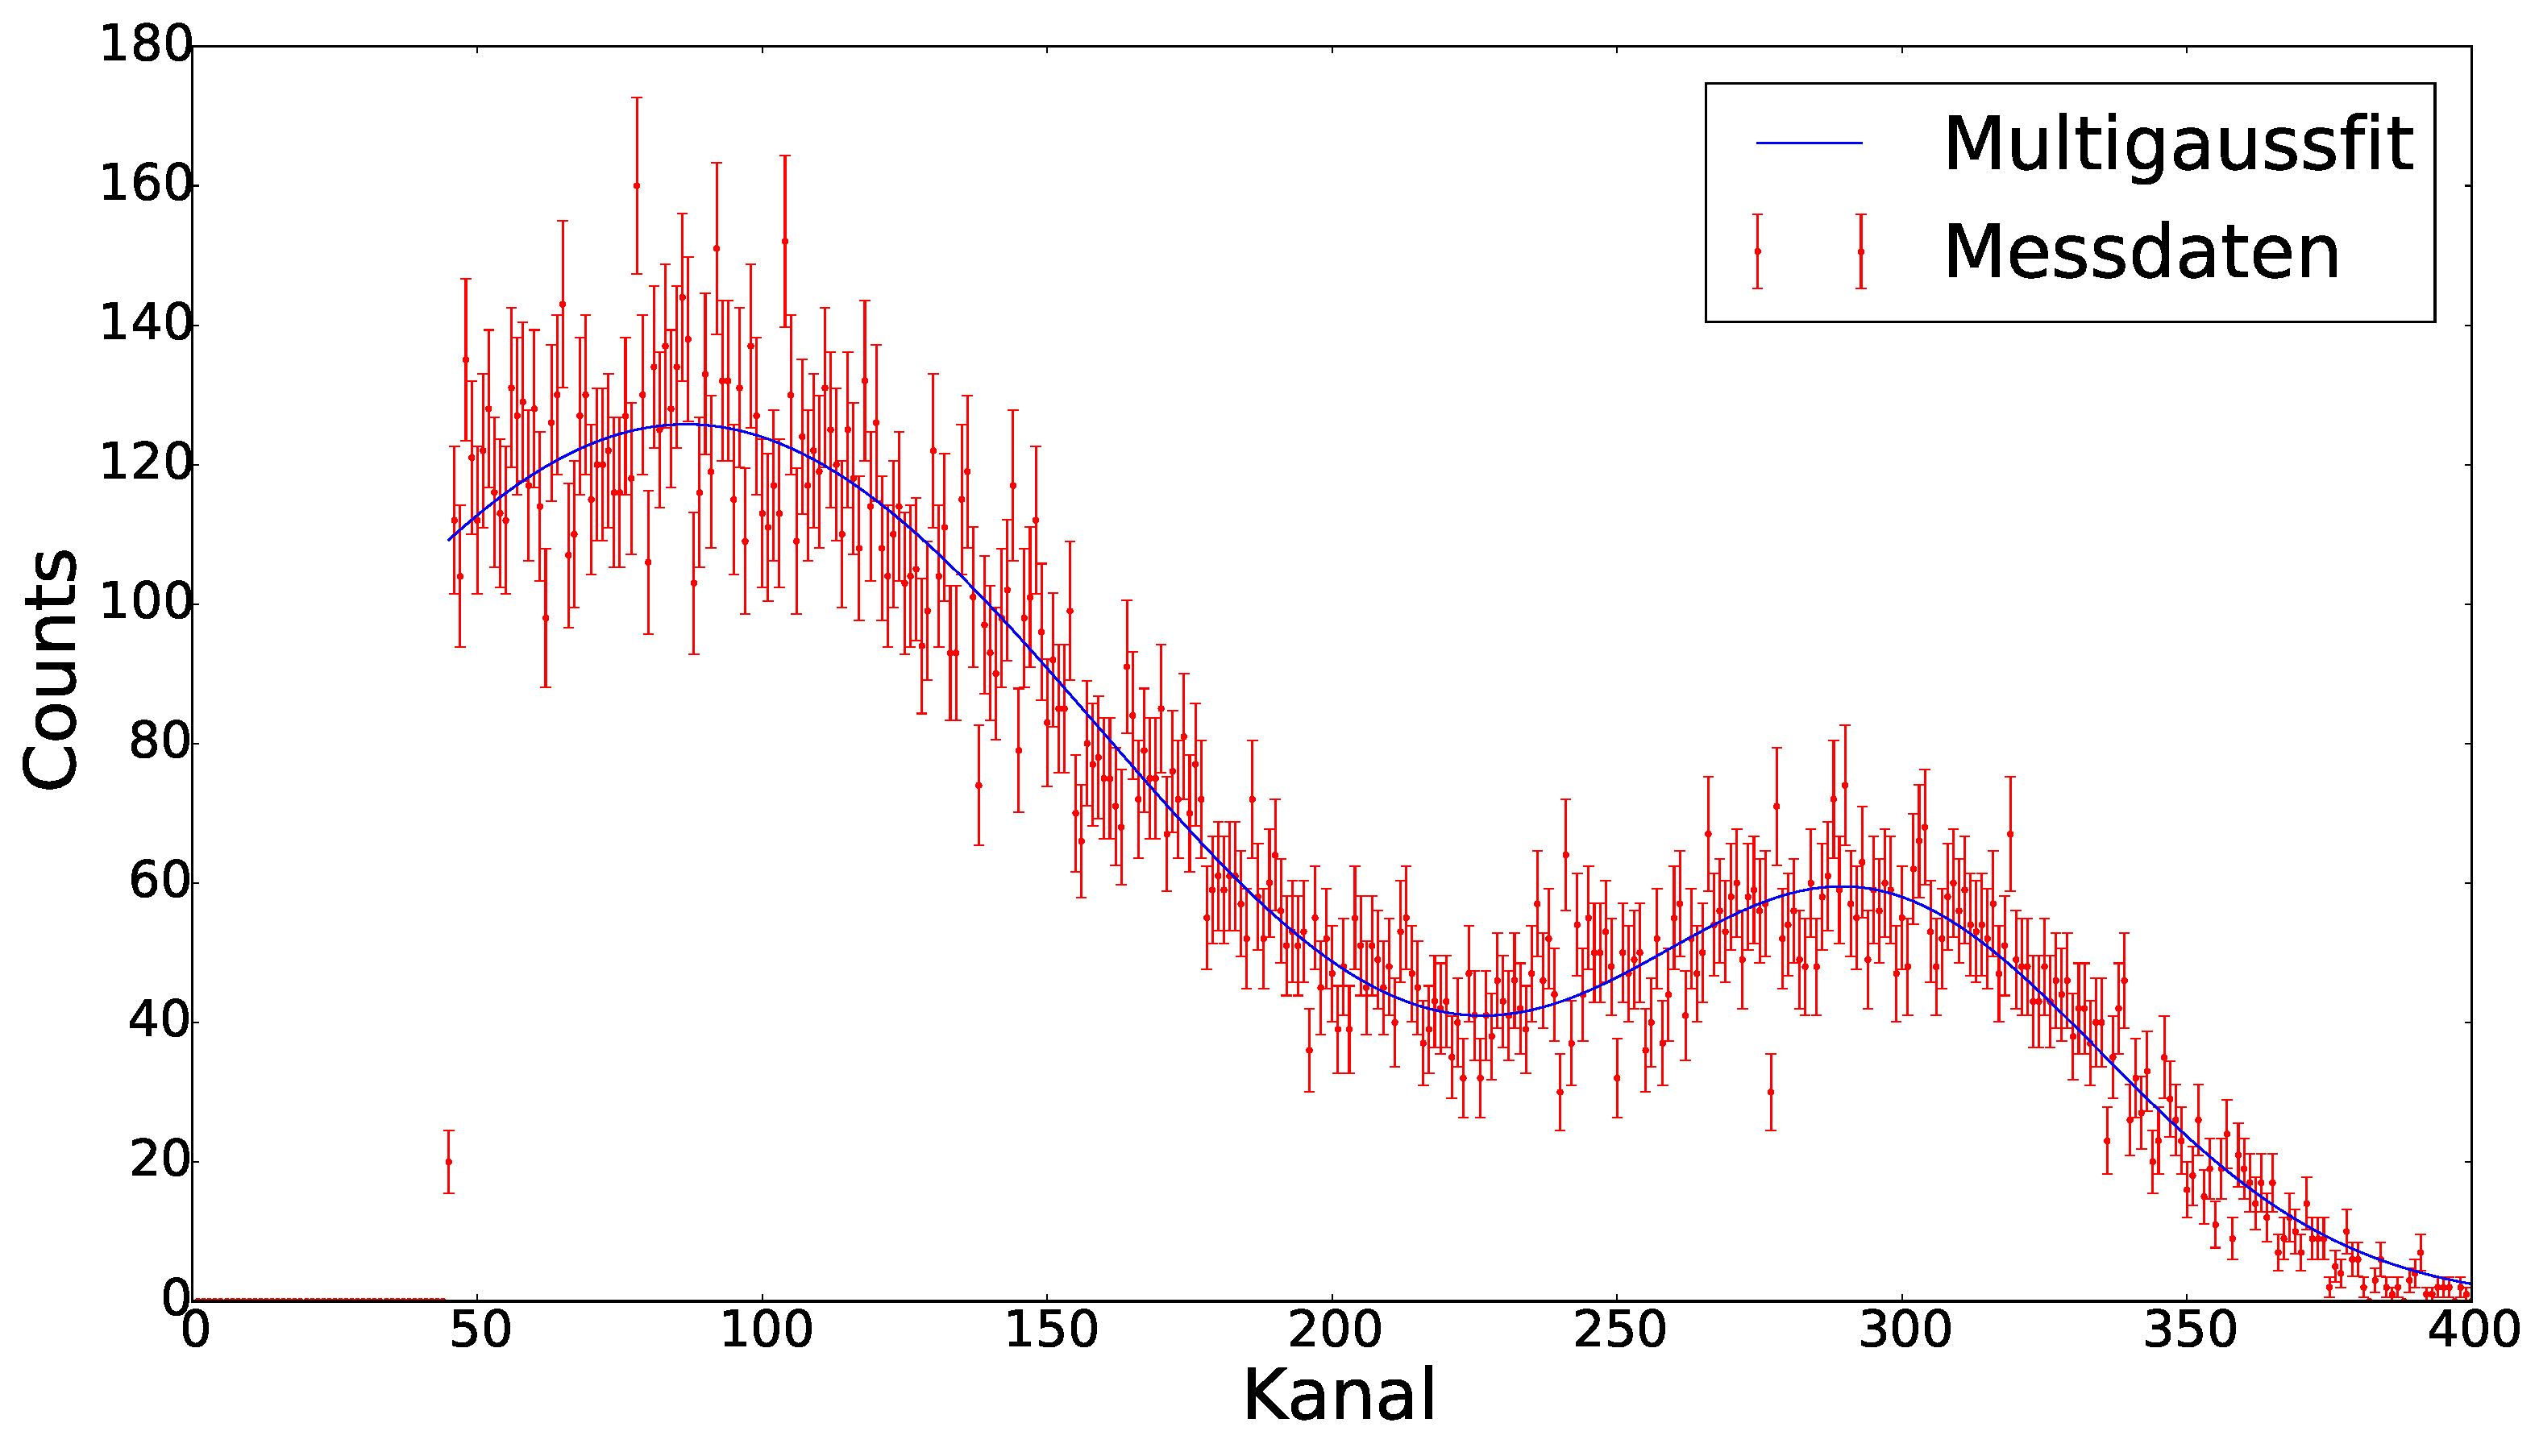
\includegraphics[scale=0.2]{ab_papier.pdf}
	\caption{Schematischer Aufbau des Streukammer}
	\label{fig:ab_papier}
\end{figure}

\begin{figure}[H]
	\centering
  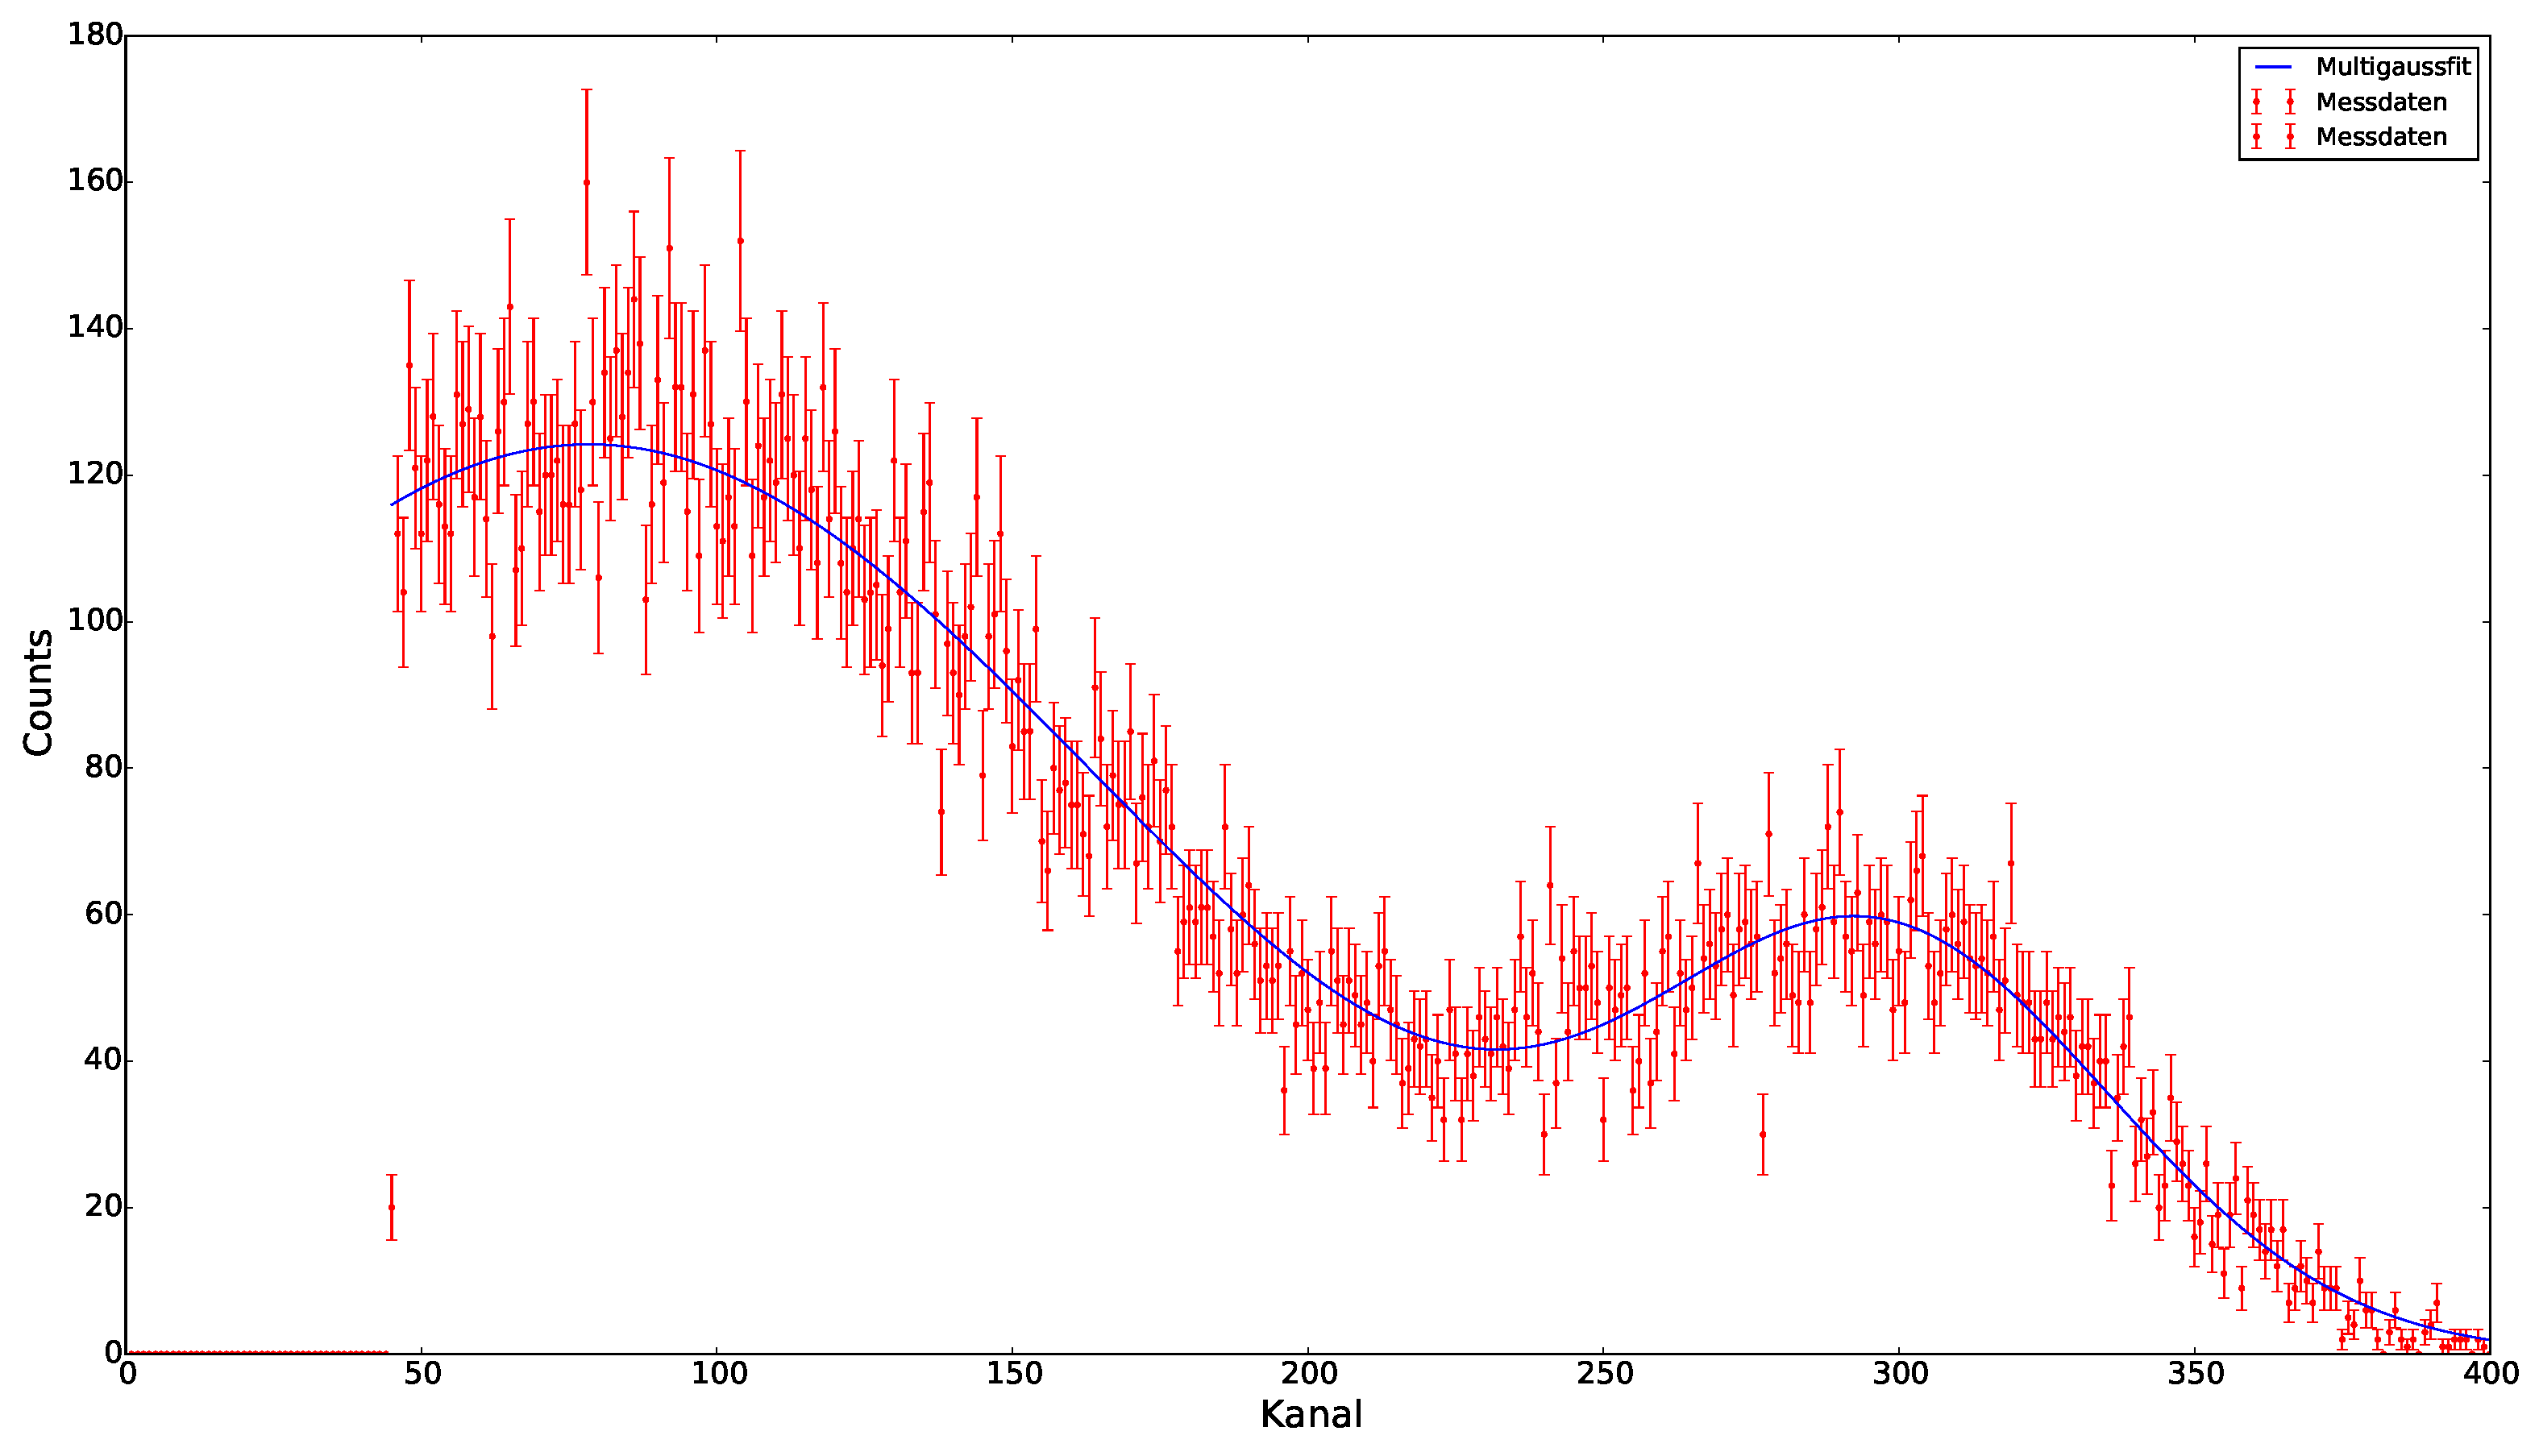
\includegraphics[scale=0.2]{ab_biebel.pdf}
	\caption{Schematischer Aufbau des Streukammer}
	\label{fig:ab_biebel}
\end{figure}

